
\documentclass[12pt]{article}
\usepackage{fullpage,amsmath,amssymb,graphicx}

\usepackage{setspace}
\spacing{1}

\usepackage{textpos}
\usepackage{tikz}
\usepackage{pgf}
\usepackage{amssymb}
\usepackage{enumerate}
\usepackage{xcolor}
\usepackage{graphicx}
\usepackage{subcaption}
\usepackage{tabularx}
\usepackage{colortbl}
\usepackage{multicol}
\usepackage{longtable}
\usepackage{hyperref}
\usepackage{comment}
\usepackage{listings}



\definecolor{encabezado}{rgb}{0.74, 0.83, 0.9}

\begin{document}

\hfill\\
\rule{\textwidth}{1.5pt}

\begin{minipage}[t]{85mm}
  \begin{tabular}{l}
    \textbf{\large Instituto Tecnológico de Costa Rica} \\  
    \textbf{Escuela de Ingeniería Electrónica} \\
    \textbf{Trabajo Final de Graduación} \\
    \textbf{Proyecto:} Método basado en aprendizaje reforzado \\para el control automático de una planta no lineal. \\
    \textbf{Estudiante:} Oscar Andrés Rojas Fonseca \hspace{3cm}\rule{4.5cm}{1.5pt}\\
    I Semestre 2024 \hspace{8.5cm}\textbf{Firma del asesor}
  \end{tabular}
\end{minipage}
\hfill\\
\rule{\textwidth}{1.5pt}


\section*{Bitácora de trabajo}

%\begin{table}[h]
\begin{minipage}[h]{\textwidth}
	\centering
	\begin{tabularx}{\textwidth}{|p{2cm}|X|X|p{2cm}|} 
		\hline
		\rowcolor{encabezado}
		\textbf{Fecha} & 
		\textbf{Actividad} & 
		\textbf{Anotaciones} & 
		\textbf{Horas dedicadas} \\ \hline
		% ***************************************************************
	 	01/05/2024 & 
	 	$\mathbf{1}.$ Reunión de seguimiento con el asesor del proyecto. & 
	 	$a)$ Revisión de avance y errores de forma. \newline
	 	$b)$ Discusión respecto al método de exploración y explotación utilizado en $PPO$. \newline & 
	 	2 horas \\
		% ***************************************************************
	 	01/05/2024 & 
	 	$\mathbf{2}.$ Entrenamiento del modelo $PPO$ y trabajo con la función $ou\_process()$. & 
	 	$a)$ Entrenamientos del modelo; comportamientos indeseados. \newline
	 	$b)$ Estudio de la función $ou\_process()$ en Octave facilitada por el profesor asesor. \newline & 
	 	6 horas \\
		% ***************************************************************
		02/05/2024 & 
	 	$\mathbf{3}.$ Adaptación de la función generación de ruido $ou\_process()$ a Python. &
	 	$a)$ Creación de la función $ou\_process()$ en $ppo_pahm.py$ al adaptarla desde Octave. \newline
	 	$b)$ Prueba de funcionamiento. Los valores base son funcionales pero requieren un mayor nivel de ruido para mover el péndulo ($sigma\approx 0.7$ funcional). \newline
	 	$c)$ Adición de la lógica para la disminución del ruido conforme el tiempo de entrenamiento. \newline & 
	 	8 horas \\
		% ***************************************************************

	 	\hline
	\end{tabularx}
\end{minipage}	 	
	 	
	 	% ***************************************************************
\hfill\\
\begin{minipage}[h]{\textwidth}
	\centering
	\begin{tabularx}{\textwidth}{|p{2cm}|X|X|p{2cm}|} 
		\hline		
		
	 	% ***************************************************************
	 	03/05/2024 & 
	 	$\mathbf{4}.$ Suma de más componentes a la observación/entrada de la red y entrenamientos $PPO$. &
	 	$a)$ Se agregó la aproximación de la velocidad angular del péndulo al $obs\_n$. \newline
	 	$b)$ Entrenamiento del modelo con la velocidad como entrada. El desempeño de la red mejoró al dejar de \textit{paralizarse} en el proceso. \newline
	 	$c)$ Se agregó la aproximación de la aceleración angular del péndulo al $obs\_n$. No se logró importante mejoría. \newline & 
	 	8 horas \\
	 	% ***************************************************************
	 	04/05/2024 & 
	 	$\mathbf{5}.$ Replanteo de la función de recompensas $calculate\_reward()$. &
	 	$a)$ Cambios de los pesos de los componentes del $reward$. \newline
	 	$b)$ Se probaron diferentes formas de plantear las ecuaciones (positivas, negativas). Los resultados demuestran el mal desempeño.  \newline & 
	 	8 horas \\
	 	% ***************************************************************
	 	05/05/2024 & 
	 	$\mathbf{6}.$ Continuación de los cambios en la función de recompensas y entrenamiento para su comprobación. &
	 	$a)$ Se utilizaron diferentes métodos y ecuaciones que al entrenar el modelo mantienen el mal desempeño. \newline & 
	 	6 horas \\
	 	% ***************************************************************
	 	07/05/2024 & 
	 	$\mathbf{7}.$ Continuación de los cambios en la función de recompensas y entrenamiento para su comprobación. &
	 	$a)$ Se consultó al asesor respecto a posibles formas de definición de la función. Se continuaron realizando pruebas con resultados indeseados. \newline & 
	 	6 horas \\
	 	% ***************************************************************
	 	
	 	\hline
		\multicolumn{3}{|r|}{Total de horas de trabajo:} & 44 horas \\ 
	 	\hline                 
	\end{tabularx}
\end{minipage}





% *****************************************************************************
% *****************************************************************************
% *****************************************************************************
\newpage

\section*{Contenidos de actividades}

La mayor parte del trabajo se enfocó en la definición de la función de recompensas, esto debido a la previa adición de los componentes de velocidad angular y aceleración del péndulo como entradas a la red neuronal, de manera que ya el agente cuenta con suficiente información para interpretar los comportamientos.

Se probaron funciones para ''castigar'' la corta duración de los episodios del $env$, dado que el comportamiento recurrente del péndulo es empujar lo suficiente para terminar rápido el episodio y no recibir tanto castigo. De manera que se probó con diferentes versiones de una función exponencial ( por ejemplo $f(x) = 1.04^{-x+50}$, Figura \ref{fig:funcion}) para castigar lo suficiente al principio del episodio y conforme avanza disminuir el castigo. El resultado fue el mismo, empujar con la se;al $PWM$ hasta terminar el episodio lo más rápido posible, ejemplificado en la Figura \ref{fig:PendPPOcaptura}

\begin{figure}[h!]
	\centering
	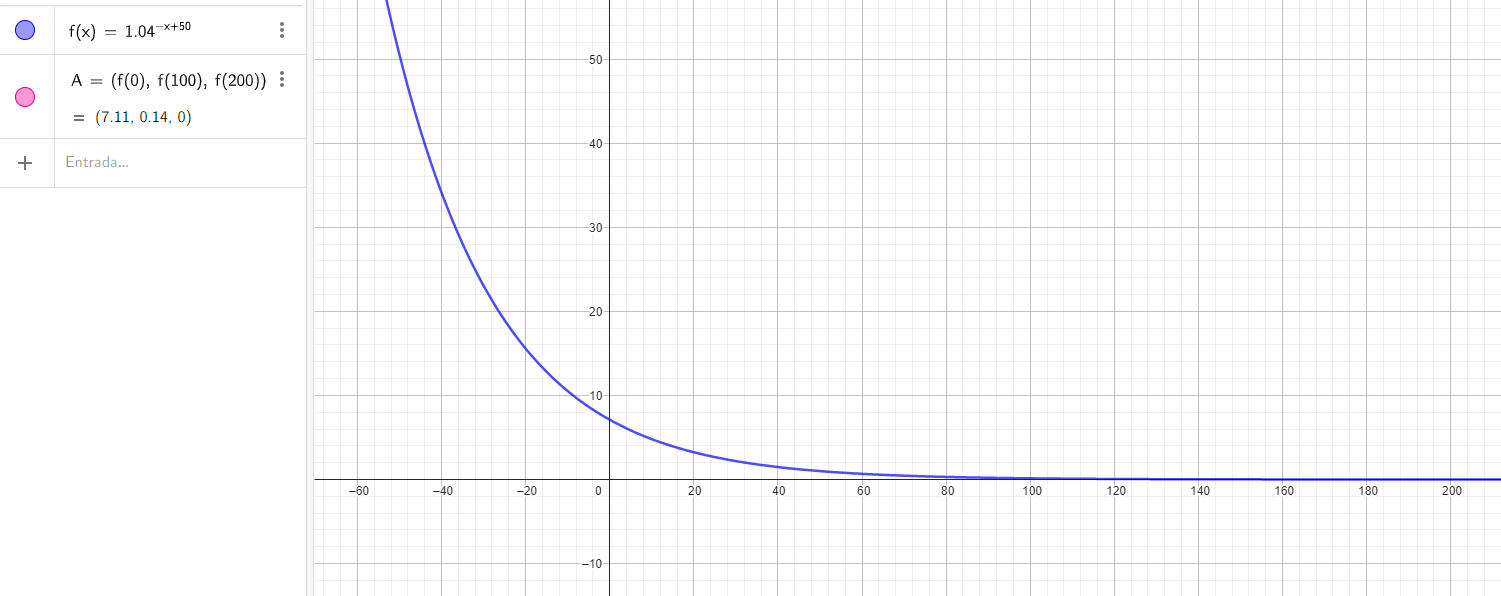
\includegraphics[scale=0.26]{Fig/Captura_funcion.png}
	\caption{Función utilizada para castigar la corta duración del episodio.}
	\label{fig:funcion}
\end{figure}	

\begin{figure}[h!]
	\centering
	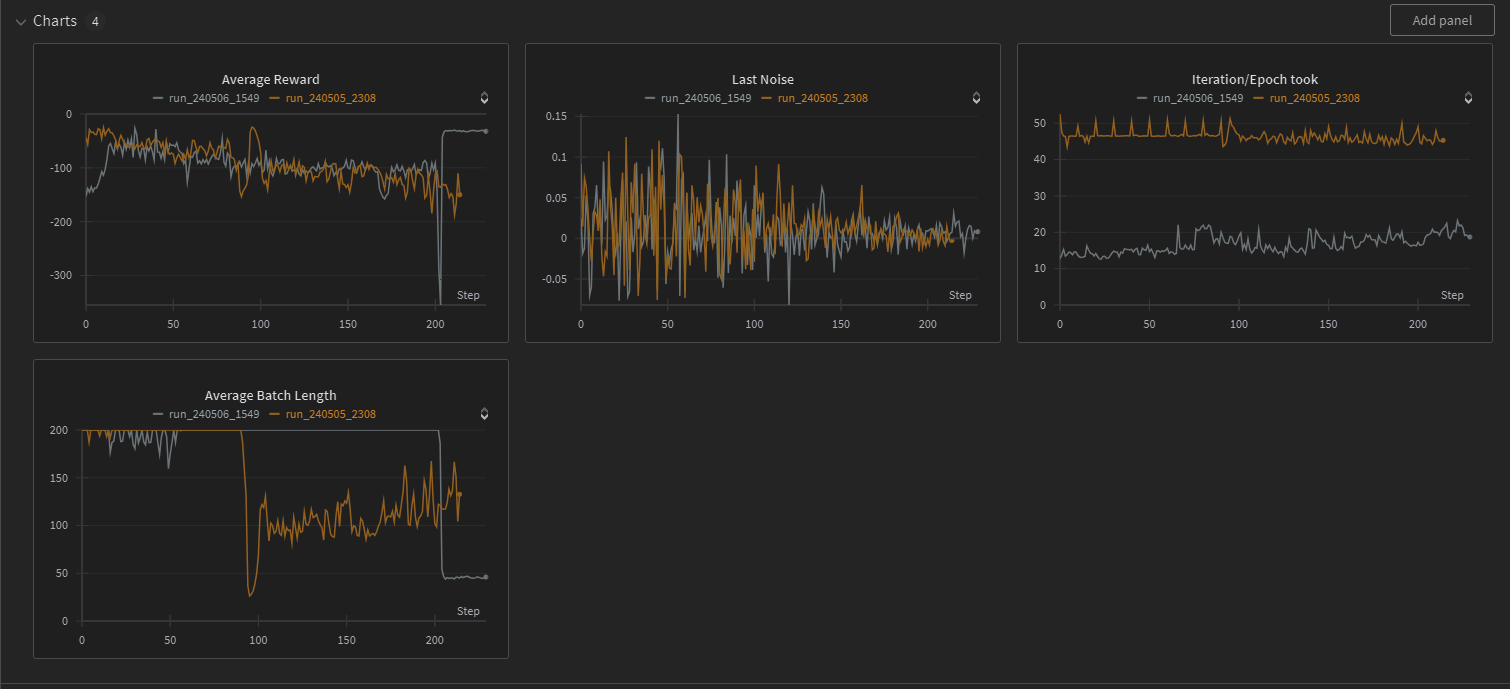
\includegraphics[scale=0.35]{Fig/Captura_entrenamientosmalos.png}
	\caption{Proceso de entrenamiento del modelo para $PendulumPPO$, resultado insatisfactorio.}
	\label{fig:PendPPOcaptura}
\end{figure}	

Se revisaron algunas de las fuentes ya consultadas como \cite{PPObeginners} con ningún avance o hallazgo significativo.

\newpage

\section*{Referencias}
\renewcommand\refname{}
\bibliographystyle{IEEEtran}
\bibliography{references}





\end{document}
